	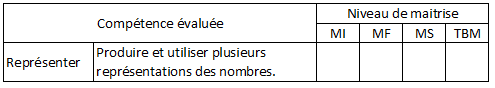
\includegraphics[scale=0.95]{competences}
	
	\section{Calculer}
	Calculer les expressions suivantes en détaillant tous les calculs:
	\begin{questions}
		
	
		\question[1]  \'Ecrire en toutes lettres le nombre \num{4580125639.245}
		
		\fillwithdottedlines{2cm}
			 
		\question[1]  \'Ecrire en chiffres le nombre cinquante-trois-milliards-huit-cent-un-millions-quarante-trois unités mille-deux-cent-vingt-cinq millièmes
		
		\fillwithdottedlines{2cm}
		
			
		
		\question[1]  \'Ecrire en chiffres le nombre cinq-cent-milliards-dix-millions-sept-cent-quarante-trois-mille unités deux-cent-soixante-quatre millièmes
		
		\fillwithdottedlines{2cm}
		
		\question[1]  Donner le chiffre des dizaines de milliers de $\num{45753438254}$
		
		\fillwithdottedlines{2cm}
	
		
		\question[1]  \'Ecrire en toutes lettres le nombre \num{5400125639.005}
		
		\fillwithdottedlines{2cm}
		
		\newpage
		
		\question[1]  Calculer $\num{45753438254} \times 1000$
		
		\fillwithdottedlines{2cm}
		
		\question[1]  Donner la nombre de dizaines de milliers de $\num{45753438254}$
		
		\fillwithdottedlines{2cm}
		
		
		\question[1]  Calculer $\num{45753438254} \div 1000$
		
		\fillwithdottedlines{2cm}
		
		
		\question[1]  Calculer $\num{38.254} \div 1000$
		
		\fillwithdottedlines{2cm}
		
		
		\question[1]  Calculer $\num{45753.438254} \times 100$
		
		\fillwithdottedlines{2cm}
		
	\end{questions}
	
	
